\icode[magenta]{E-MCH-CA-L4-261026-002}
如图，球1和球2均从同一点水平抛出，起抛点离水平地面的高度为\(H\)、两球的水平初速分别为\(v_1\)和\(v_2\)\((v_1>v_2)\)。球1抛出后刚好能越过位于\(x_P\)处的竖直杆的顶端，并落于地面上的\(R\)点，\(R\)点与\(O\)点的距离为\(R\)。球2抛出后落于地面，与地面作弹性碰撞，反弹后也刚好越过杆顶，并落在同一点\(R\)。 试求：
\begin{enumerate}
	\item \(\frac{v_1}{v_2}\)比值；
	\item 杆的位置\(x_P\)；
	\item 杆的高度\(h\)。
\end{enumerate}

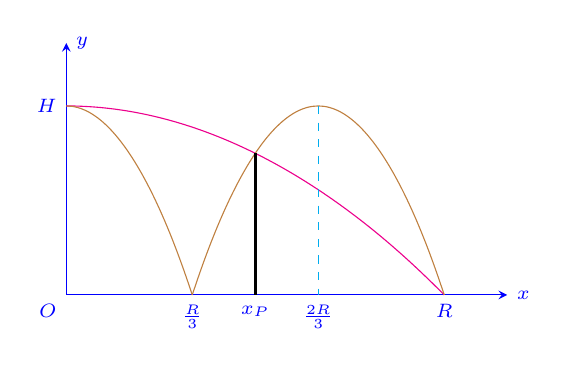
\begin{tikzpicture}[scale=.8,>=stealth,font=\scriptsize]
	\draw[->,blue] (0,0)node[below left]{ \(O\)}--(7,0)node[right]{ \(x\)};
	\draw[->,blue] (0,0)--(0,4)node[right]{ \(y\)};
	\draw[magenta] (0,3)node[left,blue]{\(H\)} parabola bend(0,3)(6,0);
	\draw[brown] (0,3) parabola bend(0,3)(2,0)node[below,blue]{\(\frac{R}{3}\)};
	\draw[brown] (2,0) parabola bend(4,3)(6,0)node[below,blue]{\(R\)};
	\draw[very thick] (3,{9/4})--(3,0)node[below,blue]{ \(x_P\)};
	\draw[dashed,cyan] (4,3)--(4,0)node[below,blue]{\(\frac{2R}{3}\)};
\end{tikzpicture}
\begin{answer}
	（1）\(3:1\)；（2）\(\frac{R}{2}\)；（3）\(\frac{3}{4}h\)\qquad 提示：注意水平分运动与竖直分运动的关系
\end{answer}